\documentclass{beamer}
%Od tukaj do polne vrstice % ne spreminjaj ničesar.
\usepackage[slovene]{babel}
\usepackage[utf8]{inputenc}
\usepackage{amsmath}
\usepackage{url}
\usepackage{graphicx}
\usepackage{tikz}
\usepackage{textpos}
\usepackage{wrapfig}

\definecolor{rdeca2017}{HTML}{8e0d1a}


\mode<presentation>
\usetheme{Boadilla}
\usefonttheme{structuresmallcapsserif}
\usenavigationsymbolstemplate{} 
\setbeamertemplate{footline}
{
  \leavevmode%
  \hbox{%
  \begin{beamercolorbox}[wd=.333333\paperwidth,ht=2.25ex,dp=1ex,center]{footline}%
    \usebeamerfont{author in head/foot}\setbeamercolor{bgcolor}{bg = rdeca2017}\insertshortauthor
  \end{beamercolorbox}%
  \begin{beamercolorbox}[wd=.333333\paperwidth,ht=2.25ex,dp=1ex,center]{footline}%
    \usebeamerfont{title in head/foot}\insertshorttitle
  \end{beamercolorbox}%
  \begin{beamercolorbox}[wd=.333333\paperwidth,ht=2.25ex,dp=1ex,right]{footline}%
    \insertframenumber{} / \inserttotalframenumber\hspace*{2ex} 
  \end{beamercolorbox}}%
  \vskip0pt%
}

\setbeamercolor{structure}{fg=rdeca2017}
\setbeamercolor{block title}{fg=white,bg=rdeca2017}
\setbeamercolor{block body}{fg=white,bg=rdeca2017}
\setbeamercolor{title}{bg = rdeca2017, fg = white}
\setbeamercolor{frametitle}{fg = white, bg = rdeca2017} 
\setbeamercolor{footline}{bg = rdeca2017, fg = white}

\addtobeamertemplate{frametitle}{}{%             %logo 
\begin{textblock*}{10mm}(.9\textwidth,-1cm)
\includegraphics[height=0.98cm]{logo_brez_ozadja.png}
\end{textblock*}}

%%%%%%%%%%%%%%%%%%%%%%%%%%%%%%%%%%%%%%%%%%%%%%
% Tukaj lahko definiraš nova okolja ali oznake.
\theoremstyle{plain}
\newtheorem{izrek}{Izrek}
\newtheorem{trditev}{Trditev}
\newtheorem{lema}{Lema}
\newtheorem{definicija}{Definicija}
% Za številske množice uporabi naslednje simbole
\newcommand{\R}{\mathbb R}
\newcommand{\N}{\mathbb N}
\newcommand{\Z}{\mathbb Z}
\newcommand{\C}{\mathbb C}
\newcommand{\Q}{\mathbb Q}

%%%%%%%%%%%%%%%%%%%%%%%%%%%%%%%%%%%%%%%%%%%%%%%
%%%%%%%%%%%%%%%%%%%%%%%%%%%%%%%%%%%%%%%%%%%%%%%
% Izpolni naslov in avtorje s svojimi podatki
\title{FUNKCIJE VEČ SPREMENLJIVK}
\author[Karmen, Žiga, Jakob, Žan]{
\includegraphics[width = 5cm]{logo_MaRS2017.png} \\ Karmen Zupančič, Žiga Flajs, Jakob Svetina \\ Mentor: Žan Hafner Petrovski}
%\date{20.~avgust~2016}

\begin{document}
%\selectlanguage{slovene}


\begin{frame}
\maketitle{FUNKCIJE VEČ SPREMENLJIVK}

\end{frame}
%%%%%%%%%%%%%%%%%%%%%%%%%%%%%%%%

\begin{frame}
\frametitle{Funkcije dveh spremenljivk}


\begin{definicija}
\textbf{Funkcija dveh neodvisnih spremenljivk} je predpis, ki vsakemu paru $(x,y)$ iz podmnožice ravnine predpiše natančno določeno realno število.
Velja torej: 
$$f : \mathbb{R}^2 \rightarrow \mathbb{R}$$
$$f:(x,y) \mapsto z=f(x,y).$$

\end{definicija}
\end{frame}


\begin{frame}
\frametitle{Primer funkcije dveh spremenljivk}
\begin{figure}[h!]
\centering
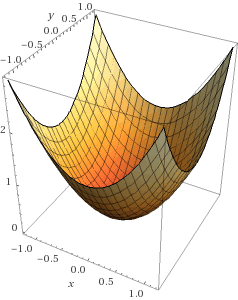
\includegraphics[width=0.4\textwidth]{slika_funkcije.PNG}
\caption{Graf funkcije $f(x,y)=x^2+y^2$}
\end{figure}
\end{frame}

\begin{frame}
\frametitle{Primer funkcije dveh spremenljivk}
\begin{figure}[h!]
\centering
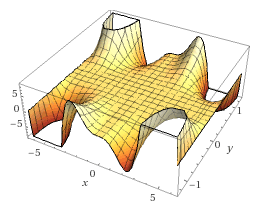
\includegraphics{funkcija_2.PNG}
\caption{Graf funkcije $g(x,y)=x^2 sin(x)y^3$}
\end{figure}
\end{frame}


%%%%%%%%%%%%%%%%%%%%%%%%%%%%%%%%
\begin{frame}
\frametitle{Polarne koordinate}
Polarni koordinatni sistem je ravninski koordinatni sistem.

\begin{figure}[h!]
\centering
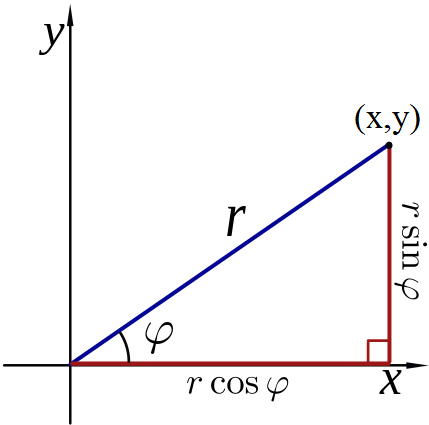
\includegraphics[width=.3\textwidth]{polarne_koordinate.png}
\caption{Grafični prikaz izražave kartezičnih koordinat s polarnimi.}
\end{figure}

\pause

Kartezični koordinati torej z $r$ in $\phi$ izrazimo takole:
\begin{itemize}
\item $x=r \cos \phi$
\item $y=r \sin \phi$
\end{itemize}
\end{frame}


\begin{frame}
\frametitle{Ploščina kroga}

Zanima nas ploščina kroga z radijem $R$.


\begin{figure}[h!]
\centering
\includegraphics[width=.3\textwidth]{krog.png}
\caption{Prikaz majhnega dela kroga.}
\end{figure}

\pause

Izračunamo integral in dobimo formulo: $$\int^{2\pi}_{0} \int^{R}_{0} r \mathrm{d} r \mathrm{d} \phi = \pi R^2$$
\end{frame}

\begin{frame}
\frametitle{Eulerjeva $\Gamma$ - funkcija}
Funkcija gama
\pause
\begin{itemize}
\item je preslikava iz $(0, \infty)$ v $\mathbb{R}$
\pause
\item za $t>0$ definirana kot: $$\Gamma(t)=\int^{\infty}_{0} x^{t-1}e^{-x} \mathrm{d} x $$
\pause
\item za $t \in [1, \infty) $ velja zveza: 
$$ \Gamma (t) = (t-1)! $$
\end{itemize}

\end{frame}


\begin{frame}
\frametitle{Eulerjeva $\Gamma$ - funkcija}
\begin{figure}
\includegraphics[width=0.57\textwidth]{graf_tock.png}
\caption{Točke na grafu so oblike $(n,(n-1)!)$ za $n \in \{1,2,3,4\}$}
\end{figure}
\end{frame}

\begin{frame}
\frametitle{Eulerjeva $\Gamma$ - funkcija}
\begin{figure}
\includegraphics[width=0.57\textwidth]{graf_desmos.png}
\caption{Graf funkcije gama}
\end{figure}
\end{frame}

%%%%%%%%%%%%%%%%
%%https://www.desmos.com/calculator/oplz8psbz4
%%https://www.desmos.com/calculator/nmufvozatc
%%https://www.probabilitycourse.com/images/chapter4/gamma-function-color.png



\end{document}















